% ------------------------------------------------------------------------------------
\vspace{5mm}
{\color{lightgray} \hrule}
\begin{enumerate}
	\item Simular $n = 5$ y $n = 50$ v.a’s Bernoulli $Be\left(\frac{1}{3}\right)$; sea $r$ el número de éxitos en cada caso.
\end{enumerate}

\textcolor{BrickRed}{\it Respuesta:}

En el archivo \textcolor{mediumblue}{ejercicio1\_tarea6.py} se implementa la función \textit{SIMULAR\_BERNOULLI()} con la cual, se simulan $n = 5$ y $n = 50$ variables aleatorias Bernoulli $Be(\frac{1}{3})$ y se calcula el número de éxitos en cada caso. Se utiliza la función \textit{np.random.binomial()} de la librería \textit{numpy} para simular las variables aleatorias binomiales ya que para el caso de una sola prueba es equivalente a una distribución Bernoulli. Se obtuvieron los siguientes resultados (se usó una semilla para reproducibilidad):
\begin{itemize}
	\item Éxitos para $n = 5: 2$.
	\item Éxitos para $n = 50: 15$.
\end{itemize}

% ------------------------------------------------------------------------------------
\vspace{5mm}
{\color{lightgray} \hrule}
\begin{enumerate} \setcounter{enumi}{1}
	\item Implementar el algoritmo Metropolis-Hastings para simular de la posterior.
	\begin{equation} \label{eq:1}
		f(p|\bar{x}) \propto p^{r} (1-p)^{n-r} \cos{(\pi p)} \cdot \mathbbm{1}_{\left[0,\frac{1}{2}\right]} (p).
	\end{equation}
	con los dos casos de $n$ y $r$ de arriba. Para ello poner la propuesta $\left(p^{'}|p\right) = p^{'} \sim Beta(r+1, n-r+1)$ y la distribución inicial de la cadena $\mu\sim\mathcal{U}\left(0,\frac{1}{2}\right)$.
\end{enumerate}

\textcolor{BrickRed}{\it Respuesta:}

En el archivo \textcolor{mediumblue}{ejercicio2\_tarea6.py} se implementa la función \textit{METROPOLIS\_HASTINGS()}, la cual simula una cadena de Markov utilizando el algoritmo de Metropolis-Hastings y toma los siguientes argumentos:
\begin{itemize}
	\item La función objetivo $f()$, (en este caso es la posterior \eqref{eq:1}).
	\item La distribución propuesta $q()$ (en este caso es la distribución $Beta(r+1, n-r+1)$).
	\item El valor inicial $x_0$ (en este caso es $\mu\sim\mathcal{U}\left(0,\frac{1}{2}\right)$.)
	\item El número de iteraciones (por default se toma $N=10000$).
\end{itemize}

Además, regresa la cadena de Markov simulada. Usa el criterio de aceptación: si $y_t$ es la propuesta dada por $q(\cdot|x_t)$ en $x_t$, entonces se acepta $y_t$ con probabilidad $\rho(x_t, y_t)$ con
\begin{equation}
	\rho(x,y) = \min\left\{1, \frac{f(y)}{f(x)} \frac{q(x|y)}{q(y|x)} \right\}
\end{equation}
y se rechada con probabilidad $1-\rho(x_t, y_t)$. A continuación, se define la función posterior \eqref{eq:1} llamada \textit{posterior()}, y la función \textit{propuesta()} dada por $Beta(r+1, n-r+1)$ la cual, como vimos en clase, no depende del estado actual $x_t$.

Finalmente, se hizo la simulación usando la función la distribución posterior \eqref{eq:1} para $n = 5$ y $n = 50$ usando el algoritmo de Metropolis-Hastings haciendo uso de la función \textit{SIMULAR\_BERNOULLI()} del ejercicio \textcolor{Purple}{1}. Se comparan las distribuciones obtenidas con un histograma y se obtuvo el siguiente resultado para una muestra de tamaño $N = 10000$:

\begin{itemize}
	\item Éxitos para $n = 5: 2$.
	\item Éxitos para $n = 50: 15$.
\end{itemize}
\begin{figure}[h!]
	\centering
	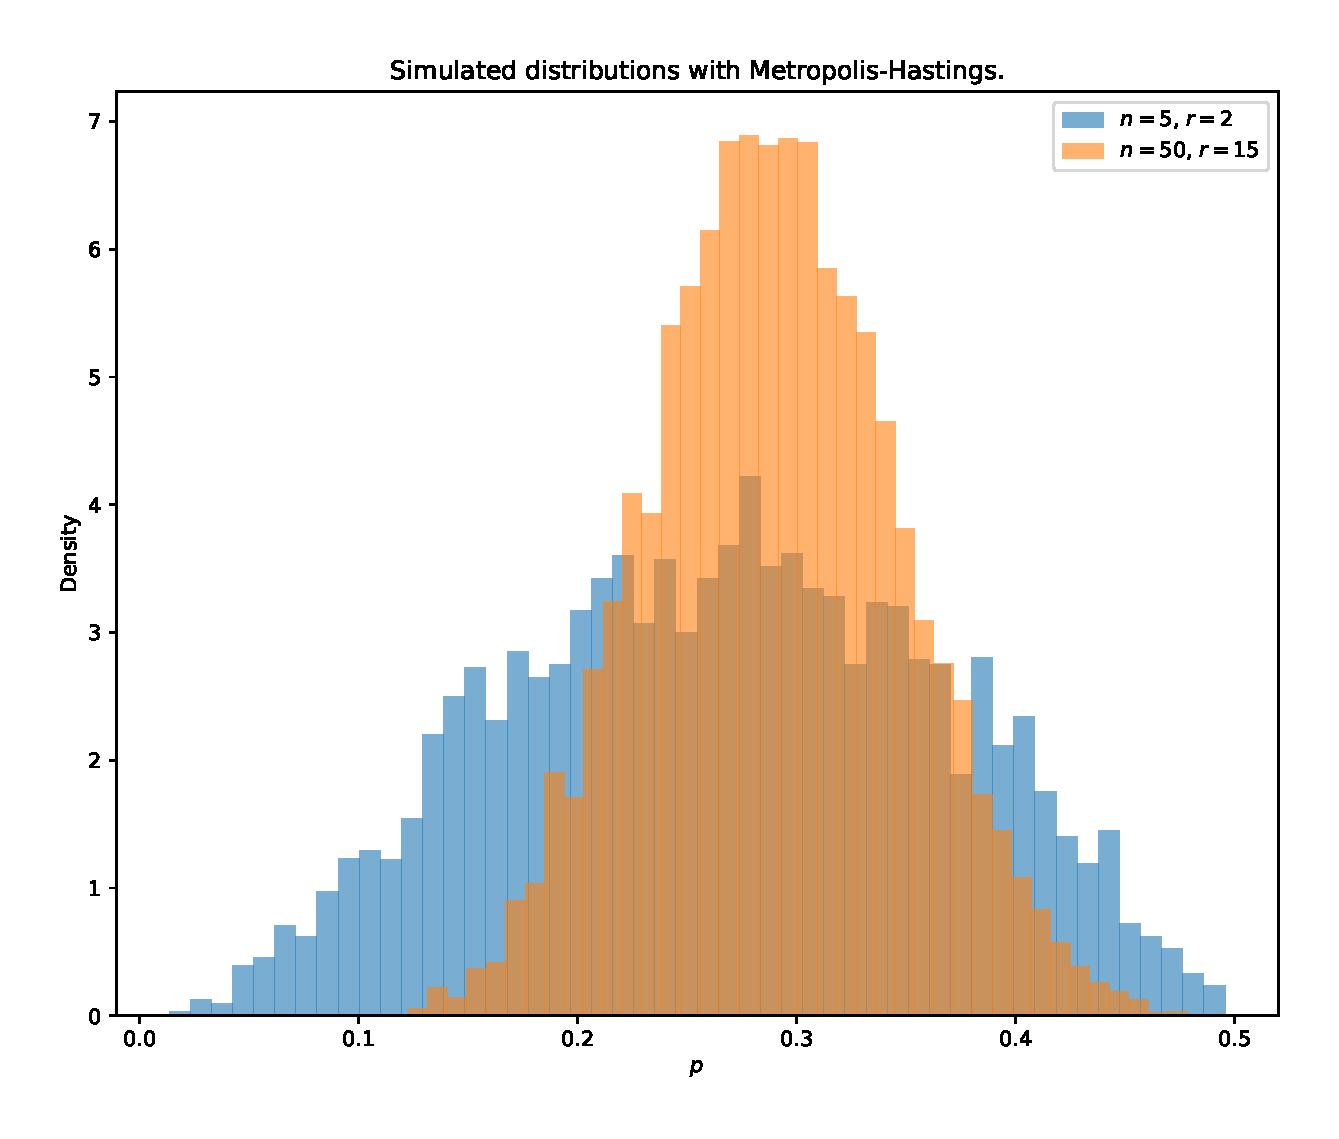
\includegraphics[width=0.85\textwidth]{IMAGENES/MS_bernoulli.pdf}
\end{figure}

Podemos notar que en ambas simulaciones para $n$ y $r$, se obtuvieron buenas estimaciones de $p = \frac{1}{3}$ ya que, $\frac{n}{r}$ no resulta tan alejado de $\frac{1}{3}$ para cada caso (se usó una semilla para reproducibilidad). 

\textcolor{red}{NOTA:} Los comentarios extras se dan al final del ejercicio \textcolor{Purple}{3}.

% ------------------------------------------------------------------------------------
\vspace{5mm}
{\color{lightgray} \hrule}
\begin{enumerate} \setcounter{enumi}{2}
	\item Argumentar porque la cadena es $f-$irreducible y porque es ergódica. Implementar el algoritmo con los datos descritos y discutir los resultados.
\end{enumerate}

\textcolor{BrickRed}{\it Respuesta:}

Sabemos que la $f-$irreducibilidad de una cadena de Markov significa que es posible alcanzar cualquier subconjunto del espacio de estados a partir de cualquier estado con probabilidad positiva, donde  $f$  es una medida no trivial en el espacio de estados. En el contexto del algoritmo Metropolis-Hastings con nuestra propuesta
\begin{equation}
	 p^{'} | p \sim Beta(r+1, n-r+1), 
\end{equation}
la cadena es  $f-$irreducible por las siguientes razones:
\begin{itemize}
	\item \textbf{Soporte de la propuesta:} La distribución $Beta(r+1, n-r+1)$ tiene soporte en $[0, 1]$  (aunque la posterior tiene soporte restringido a $[0, \frac{1}{2}]$ y claramente $[0, \frac{1}{2}] \subset [0, 1]$). Esto significa que, desde cualquier valor  $p \in (0, \frac{1}{2})$, la propuesta tiene probabilidad positiva de moverse a cualquier otro punto en este intervalo.
	
	\item \textbf{Aceptación de la propuesta:} La densidad objetivo $f(p|\bar{x})$ es continua y positiva en el intervalo $(0, \frac{1}{2})$ (aunque puede ser cercana a cero en los extremos). Esto asegura que hay una probabilidad positiva de aceptar cualquier propuesta $p^{'} | p$ si proviene de la distribución $Beta(r+1, n-r+1)$, siempre que esté dentro de $(0, \frac{1}{2})$.
\end{itemize}

Por lo tanto, desde cualquier estado $p$ , es posible alcanzar cualquier otro estado en $(0, \frac{1}{2})$ con probabilidad positiva, lo que asegura que la cadena es  $f-$irreducible $_\blacksquare$

Ahora, la ergodicidad de la cadena se refiere a que, con el tiempo, la cadena “visita” todos los estados posibles de manera que las frecuencias de visita convergen a las probabilidades estacionarias de la distribución objetivo $f(p|\bar{x})$. En clase revisamos que, el que la cadena sea $f-$irreducible entonces era ergódica, sin embargo, se va a detallar más:

La cadena es ergódica por las siguientes razones:
\begin{itemize}
	\item \textbf{Irreducibilidad:} Ya se revisó que la cadena es $f-$irreducible, lo que es una condición necesaria para la ergodicidad.
	\item \textbf{Aperiodicidad:} La propuesta Beta no es determinista, lo que implica que no hay ciclos predefinidos en la cadena. Esto significa que la cadena no quedará atrapada en patrones cíclicos, y por tanto es aperiodica (en clase vimos que dada la aperiodicidad, la cadena convergía a la distribución objetivo).
	\item \textbf{Acotamiento del soporte:} La posterior \eqref{eq:1} tiene soporte en $[0, \frac{1}{2}]$, lo que es un conjunto acotado. En este intervalo, la distribución Beta y la densidad objetivo permiten que la cadena se mueva de manera adecuada por todo el espacio, y la distribución $f(p|\bar{x})$ actúa como la distribución estacionaria $_\blacksquare$
\end{itemize}

\textcolor{red}{Resultados:} 

Ya se implementó el algoritmo con los datos descritos en el ejercicio anterior en el archivo \textcolor{mediumblue}{ejercicio2\_tarea6.py} y se tienen los siguientes resultados/comentarios.

Como se mencionó antes, se puede notar que en ambas simulaciones para $n$ y $r$, se obtuvieron buenas estimaciones de $p = \frac{1}{3}$ ya que, $\frac{n}{r}$ no resulta tan alejado de $\frac{1}{3}$ para cada caso. Variando la semilla, se notó en algunas ocasiones un mal desempeño al momento de estimar $p=\frac{1}{3}$, esto dependiento de la simulación de $r$ para $n = 5$  o $n = 50$, ya que para ser un mejor estimador, $r$ debe ser $\frac{n}{3}$ aproximadamente. Un ejemplo de esto se puede ver en la siguiente figura:

Además, cuando $n$ es pequeño (como $n=5$), la distribución simulada tiende a estar más dispersa. Esto se debe a que la cantidad de datos disponibles ($5$) no es suficiente para ajustar fuertemente los parámetros de la posterior. Cuando $n$ es mayor, la distribución se ajusta más cerca de los valores que maximizan la posterior, lo que refleja una mayor precisión en la estimación del parámetro $p$ debido a la mayor cantidad de datos.

Finalmente, dado que la cadena es ergódica, tras un número suficientemente grande de iteraciones, las muestras convergen a la distribución posterior $f(p|\bar{x})$. Esto se observa en la forma de los histogramas que se alinean con las formas teóricas esperadas de las distribuciones.

\begin{figure}[h!]
	\centering
	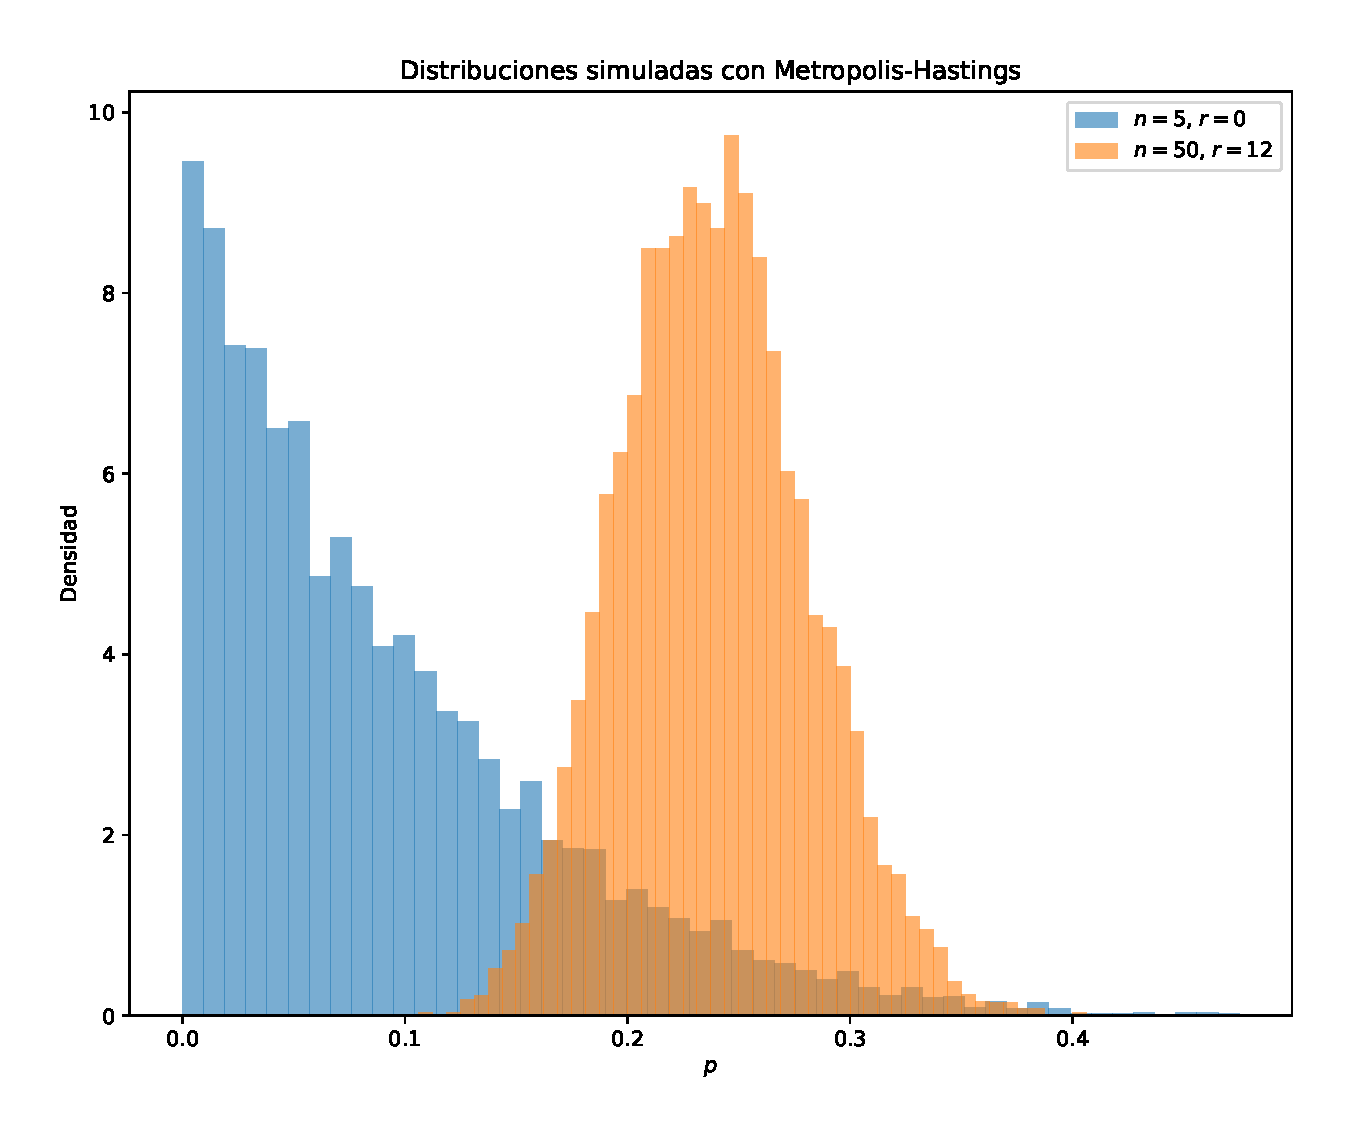
\includegraphics[width=0.85\textwidth]{IMAGENES/posteriormala.pdf}
\end{figure}

% ------------------------------------------------------------------------------------
\vspace{5mm}
{\color{lightgray} \hrule}
\begin{enumerate} \setcounter{enumi}{3}
	\item Implementar el algoritmo Metropolis-Hastings con la posterior de arriba tomando una propuesta diferente.
\end{enumerate}

\textcolor{BrickRed}{\it Respuesta:}

Dentro de la bibliografía más importante relacionada con Metropolis-Hastings, se encontró que un ejemplo común de propuesta es usar una distribución normal simétrica alrededor del valor actual $p$, como 
\begin{equation} \label{eq:4}
	p^{'}|p \sim \mathcal{N}(p, \sigma^2) ,
\end{equation}
truncada en el intervalo $[0, \frac{1}{2}]$. Esto garantiza que las propuestas siempre estén dentro del dominio de la posterior. En el archivo \textcolor{mediumblue}{ejercicio4\_tarea6.py} se usa la misma estructura del programa implementado en el ejercicio \textcolor{Purple}{2}, con la diferencia de que se modificó la propuesta $\left(p^{'}|p\right) = p^{'} \sim Beta(r+1, n-r+1)$ por \eqref{eq:4} con $\sigma^2=	0.1$ para controlar la dispersión de las propuestas.

Se usó la misma distribución inicial de la cadena $ \mu \sim \mathcal{U} \left( 0, \frac{1}{2} \right)$ y se obtuvieron los siguientes resultados:

\begin{itemize}
	\item Éxitos para $n = 5: 2$.
	\item Éxitos para $n = 50: 15$.
\end{itemize}

Además, experimentando con varias configuraciones, como variando el parámetro $\sigma^2$ y el número de muestras $n$, se pudo notar que, al igual que antes cuando $n$ crece, se tiene que la distribución se ajusta más cerca de los valores que maximizan la posterior, lo que refleja una mayor precisión en la estimación del parámetro $p$ debido a la mayor cantidad de datos y que funciona mejor con un valor de $\sigma^2$ pequeño. Se puede notar que la distribución propuesta \eqref{eq:4}, también cumple con las condiciones que hacen que la cadena sea $f-$irreducible y ergódica por las mismas razones mencionadas en el ejercicio \textcolor{Purple}{3}.
\begin{figure}[h!]
	\centering
	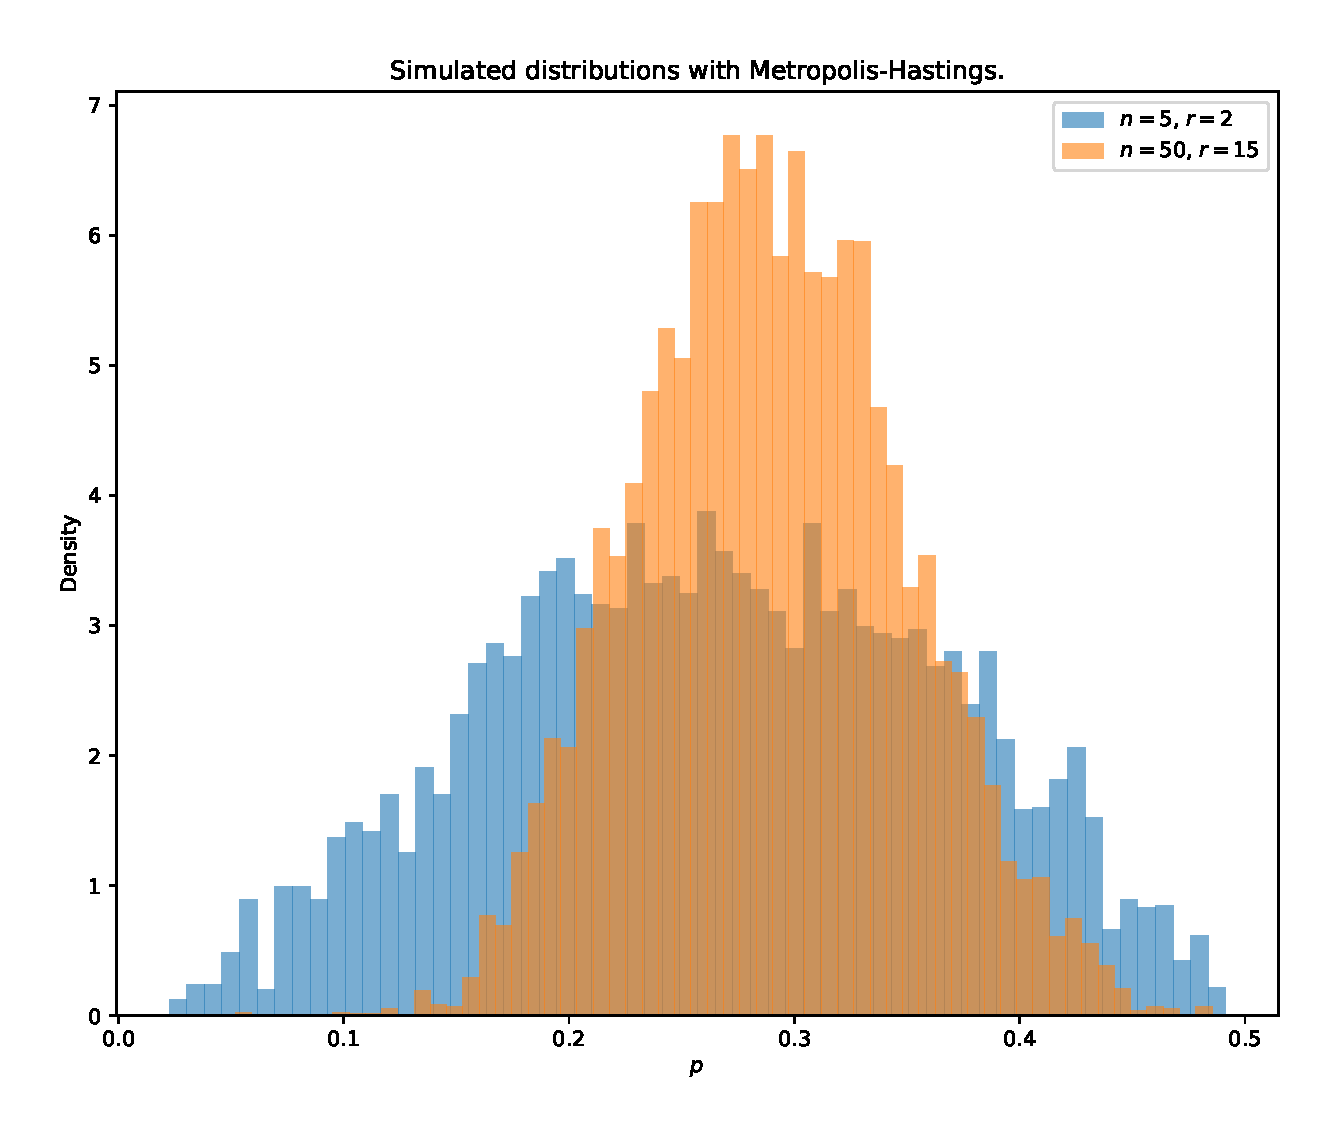
\includegraphics[width=0.85\textwidth]{IMAGENES/MS_normal.pdf}
\end{figure}




